\documentclass[letterpaper,journal]{IEEEtran}
\usepackage{amsmath,amsfonts}
\usepackage{algorithmic}
\usepackage{array}
\usepackage{graphicx}
\graphicspath{{img/}}
\usepackage{float}
\usepackage[caption=false,font=normalsize,labelfont=sf,textfont=sf]{subfig}
\usepackage{textcomp}
\usepackage{stfloats}
\usepackage{url}
\usepackage{verbatim}
\usepackage{cite}
\usepackage{multirow}
\usepackage{booktabs}

\begin{document}

\title{ECE 276B Project 2: Motion Planning}
\author{Dong-Yue Chang} % 這邊我稍後自己填

\maketitle

% ==========================================
% 1. Introduction
% ==========================================
\section{Introduction}
Motion planning is a fundamental capability in autonomous robotics that enables systems to navigate complex environments by finding safe trajectories from a start state to a goal state. In this project, we address the challenge of designing algorithms for motion planning to both static and dynamic goals in continuous three dimensional Euclidean space. The environments are defined by a rectangular outer boundary and populated with obstacles represented as axis aligned bounding boxes.

To ensure the safety of the planned trajectories, we first implement a robust algorithm for checking intersections between continuous line segments and the obstacle boxes. Building upon this foundation, we develop a sampling based planning approach utilizing the Rapidly Exploring Random Tree algorithm to compute efficient paths in environments with static goals.

Furthermore, we extend our approach to handle fast replanning scenarios where a target moves through eight goal positions in sequence. Because the target remains at each position for only a strictly limited amount of time, our planner is optimized to quickly compute paths to the current goal before the target transitions to the next, all without utilizing future goal locations in advance. This report details the mathematical problem formulation, the design and optimization of our technical approach, and a comprehensive evaluation of the performance of the algorithms in both static and dynamic settings.

% ==========================================
% 2. Problem Formulation
% ==========================================
\section{Problem Formulation}
The motion planning problem for this project is formulated by extending the finite-state Deterministic Shortest Path (DSP) problem to a continuous 3-D configuration space. Based on the formal definitions of sampling-based motion planning, we establish the following foundational elements:

\begin{itemize}
    \item \textbf{Configuration Space:} Let the configuration space be $\mathcal{C} \subset \mathbb{R}^3$, which is bounded by a predefined rectangular outer boundary.
    \item \textbf{Obstacle Space:} The obstacle space $\mathcal{C}_{obs} \subset \mathcal{C}$ consists of a set of static, axis-aligned bounding boxes (AABBs). Each obstacle is mathematically defined by a 9-dimensional vector specifying its lower-left corner $(x_{min}, y_{min}, z_{min})$, its upper-right corner $(x_{max}, y_{max}, z_{max})$, and its RGB color for visualization.
    \item \textbf{Free Space:} The valid planning domain, where navigation is permitted without collision, is defined as the free space $\mathcal{C}_{free} = \mathcal{C} \setminus \mathcal{C}_{obs}$.
    \item \textbf{Path:} A path is defined as a continuous function $\rho: [0, 1] \rightarrow \mathcal{C}$.
    \item \textbf{Feasible Path:} A feasible path is a continuous function $\rho: [0, 1] \rightarrow \mathcal{C}_{free}$ such that $\rho(0) = x_s$ and $\rho(1) = x_\tau$, where $x_s \in \mathcal{C}_{free}$ is the start state and $x_\tau \in \mathcal{C}_{free}$ is the goal state. The set of all feasible paths from $x_s$ to $x_\tau$ is denoted as $\mathcal{P}_{s, \tau}$.
\end{itemize}

\subsection{Static Goal Planning}
For environments with a static target, the motion planning problem is stated as follows: Given the free space $\mathcal{C}_{free}$, the obstacle space $\mathcal{C}_{obs}$, a start state $x_s$, a goal state $x_\tau$, and a cost function $J: \mathcal{P} \rightarrow \mathbb{R}_{\ge 0}$ (representing the Euclidean path length), the objective is to find an optimal feasible path $\rho^*$ such that:
\begin{equation}
    J(\rho^*) = \min_{\rho \in \mathcal{P}_{s, \tau}} J(\rho)
\end{equation}
or report failure if no such path exists.

\subsection{Dynamic Fast Replanning}
For the fast replanning scenario, the problem is extended to an incremental search problem. Instead of a single static goal, the target moves through a sequence of eight goal positions, $x_{\tau, 1}, x_{\tau, 2}, \dots, x_{\tau, 8}$. The planner must compute a feasible path $\rho_k^*$ from the initial start state $x_s$ to the current goal $x_{\tau, k}$ under strict computation time constraints. Specifically, the target remains at the first goal for a limited duration $t_1$, and at subsequent goals for a duration $t_2$.

Because information about future goal locations cannot be utilized in advance, the problem requires solving a series of sequential shortest path queries. To satisfy the strict time bounds $t_1$ and $t_2$, the solver must either optimize its efficiency to plan from scratch within the time limit (acting as an anytime planner), or utilize incremental search techniques (such as concepts from $LPA^*$ or $D^*$ Lite) to reuse prior search information—such as explored nodes, sampled points, or cost-to-arrive values—from previous planning queries.


% ==========================================
% 3. Technical Approach
% ==========================================
\section{Technical Approach}
\subsection{Collision Checking}
According to the principles of configuration space, once the obstacles are defined in the workspace, planning can be executed for a point robot, which makes collision checking highly efficient. Instead of explicitly pre-computing a dense representation of the configuration space, our planner performs collision checking on the fly by evaluating line segments directly against the obstacle boundaries.

To evaluate the safety of the planning algorithm, we implement a continuous 3-D collision checking algorithm between line segments and axis aligned bounding boxes (AABBs). We utilize the robust Slab Method (Ray-AABB Intersection) for its computational efficiency, which is critical for sampling based planners that require thousands of collision queries.

First, alternative approaches such as naive point discretization (evaluating discrete points along a segment) suffer from severe performance bottlenecks. Evaluating thousands of generated segments against multiple obstacles using iterative loops creates a computational disaster, making it nearly impossible to meet the strict 0.1 second fast replanning constraint required for the dynamic target in Part 3. The Slab Method, in contrast, enables purely vectorized matrix operations, allowing simultaneous evaluation of a single segment against all obstacles with minimal overhead.

Second, while the project guidelines permit the utilization of existing external collision detection libraries, integrating heavy external dependencies often introduces complex environment bindings and compilation issues. By natively implementing the Slab Method, we maintain a lightweight, completely self contained codebase that is perfectly optimized for the specific obstacle format provided in the environments.

Let a line segment be defined by a start point $p_1 \in \mathbb{R}^3$ and an end point $p_2 \in \mathbb{R}^3$. We parameterize the segment as a ray with origin $O = p_1$ and direction vector $D = p_2 - p_1$. Any point on the segment can be evaluated by $P(t) = O + tD$, where $t \in [0, 1]$.

Each AABB is defined by its minimum bounds $B_{min} = (x_{min}, y_{min}, z_{min})$ and maximum bounds $B_{max} = (x_{max}, y_{max}, z_{max})$. For each axis $i \in \{x, y, z\}$, we compute the intersection parameters with the parallel slabs defining the AABB:
\begin{equation}
    t_{min, i} = \frac{B_{min, i} - O_i}{D_i}, \quad t_{max, i} = \frac{B_{max, i} - O_i}{D_i}
\end{equation}
To account for negative direction components, we ensure $t_{min, i} \le t_{max, i}$ by swapping them if $D_i < 0$. The overall intersection interval along the ray is determined by the intersection of the intervals for all three axes:
\begin{equation}
    t_{enter} = \max_i (t_{min, i}), \quad t_{exit} = \min_i (t_{max, i})
\end{equation}
A collision occurs if and only if the segment intersects the bounding box, which corresponds to the condition:
\begin{equation}
    t_{enter} \le t_{exit} \quad \text{and} \quad t_{exit} \ge 0 \quad \text{and} \quad t_{enter} \le 1
\end{equation}
If this condition holds, the line segment intersects the $\mathcal{C}_{obs}$ space, and the connection is deemed invalid. By utilizing vectorized operations for this procedure, we can evaluate a single segment against all $N$ obstacles simultaneously, drastically reducing the overhead during the graph construction phase.

\subsection{Fast Replanning Strategy}
For environments with a dynamic target (Part 3), the planner must compute a trajectory to eight sequential goal positions within strict time limits. Specifically, in the Room environment, the planner is restricted to 0.3 seconds for the first goal and 0.1 seconds for subsequent goals. Instead of reusing information from previous search trees via incremental search techniques like $D^*$ Lite, our approach tackles the fast replanning problem by executing a completely new search from scratch for each goal transition.

To achieve the extreme computational efficiency required to meet these deadlines, our implementation relies on the synergy of vectorized collision checking and goal-biased sampling. By allocating static memory arrays for the tree nodes upfront, we eliminate the overhead of dynamic memory allocation during the high frequency Python execution loop.

Furthermore, the 10 percent goal bias aggressively directs the tree toward the current target, bypassing exhaustive free space exploration. Because we do not utilize future goal locations in advance, the planner must be purely reactive. This combination allows the optimized vanilla Rapidly Exploring Random Tree to routinely find a valid path within milliseconds. Our approach demonstrates that a highly optimized, memory contiguous standard planner can effectively satisfy stringent time limits without incurring the structural maintenance overhead required by complex incremental algorithms.

\subsection{Algorithmic Evolution and Overcoming Bug Traps}
During the development phase, we initially deployed a unidirectional Rapidly Exploring Random Tree equipped with a ten percent goal-biased sampling strategy. The primary motivation was to meet the extreme dynamic replanning constraints of Part 3. While this initial planner achieved millisecond execution times in open spaces like the Room environment, it suffered catastrophic failures in highly constrained spaces.

Specifically, when tested in the Maze environment (Environment 2), the aggressive goal directed heuristic repeatedly forced the tree into local minima, effectively trapping the planner in what is commonly known as a bug trap. The unidirectional tree would exhaust its iteration limits by continuously attempting to penetrate solid walls toward the goal, failing to explore alternative escape routes through the narrow corridors.

To resolve this critical vulnerability, we transitioned the primary architecture to the Bi-Directional RRT-Connect algorithm. By growing two trees simultaneously from both the start and goal configurations, and replacing the manual goal bias with a greedy bidirectional connection heuristic, the algorithm naturally balances rapid exploration with goal directed convergence. This architectural upgrade proved highly successful: the RRT-Connect algorithm seamlessly escaped the bug traps in the Maze environment, finding a valid solution in approximately 6.7 seconds, while simultaneously maintaining the sub 0.1 second replanning speeds required for the dynamic targets in Part 3.

Both planner implementations are preserved in the submitted codebase to demonstrate this algorithmic progression.
% ==========================================
% 4. Results
% ==========================================
\section{Results and Discussion}
In this section, we comprehensively evaluate the Bi-Directional RRT-Connect planner across all seven test environments. The algorithm successfully generated collision free trajectories with a one hundred percent success rate.

\subsection{Static Goal Environments}
The planner was tested on five static environments: Single Cube, Flappy Bird, Tower, Maze, and Monza. Table \ref{tab:static_results} summarizes the computation times and total path lengths for each scenario. The algorithm demonstrates exceptional speed in open spaces while maintaining robust performance in highly constrained spaces like Maze and Monza, effectively overcoming bug traps.

\begin{table}[htbp]
    \caption{Performance in Static Environments}
    \begin{center}
        \begin{tabular}{|c|c|c|}
            \hline
            \textbf{Environment} & \textbf{Planning Time (s)} & \textbf{Path Length} \\
            \hline
            Single Cube          & 0.008                      & 8.0                  \\
            \hline
            Flappy Bird          & 0.072                      & 42.0                 \\
            \hline
            Tower                & 0.195                      & 46.0                 \\
            \hline
            Maze                 & 2.840                      & 106.0                \\
            \hline
            Monza                & 5.025                      & 105.0                \\
            \hline
        \end{tabular}
        \label{tab:static_results}
    \end{center}
\end{table}

Figures \ref{fig:single_cube} through \ref{fig:monza} visualize the successful 3D trajectories generated for all static environments.

\begin{figure}[htbp]
    \centerline{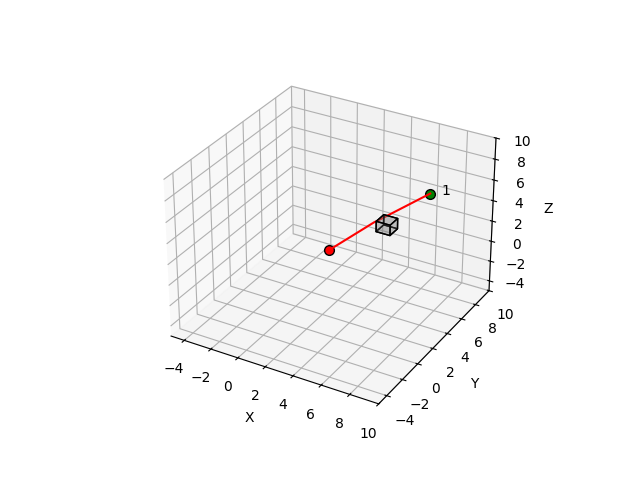
\includegraphics[width=0.7\columnwidth]{test_single_cube.png}}
    \caption{Trajectory in the Single Cube environment.}
    \label{fig:single_cube}
\end{figure}

\begin{figure}[htbp]
    \centerline{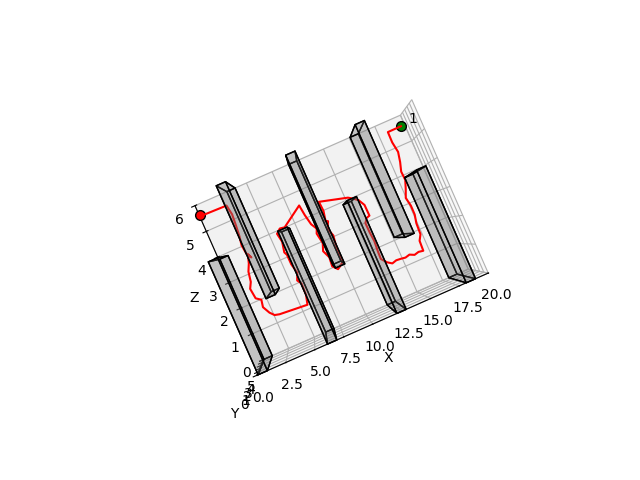
\includegraphics[width=0.7\columnwidth]{test_flappy_bird.png}}
    \caption{Trajectory navigating through the Flappy Bird environment.}
    \label{fig:flappy_bird}
\end{figure}

\begin{figure}[htbp]
    \centerline{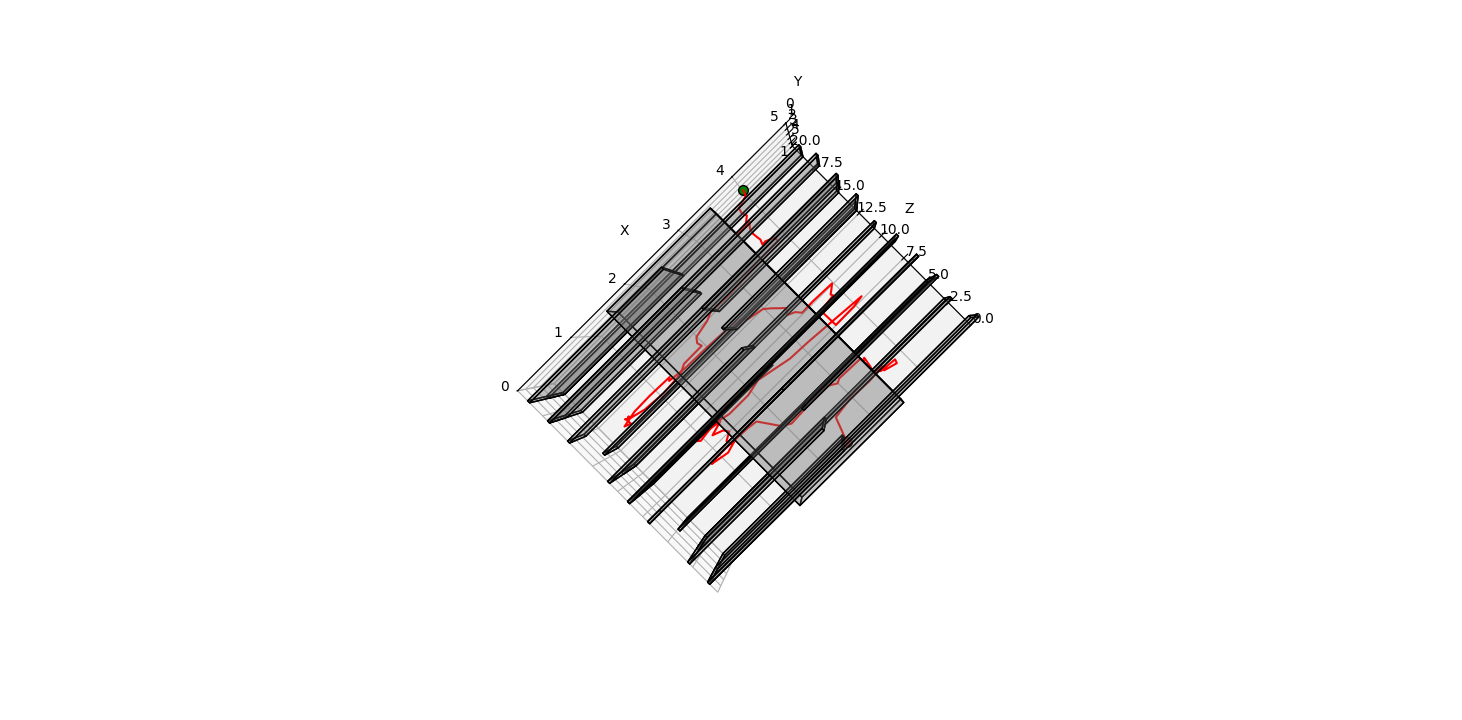
\includegraphics[width=0.7\columnwidth]{test_tower.png}}
    \caption{Trajectory ascending the Tower environment.}
    \label{fig:tower}
\end{figure}

\begin{figure}[htbp]
    \centerline{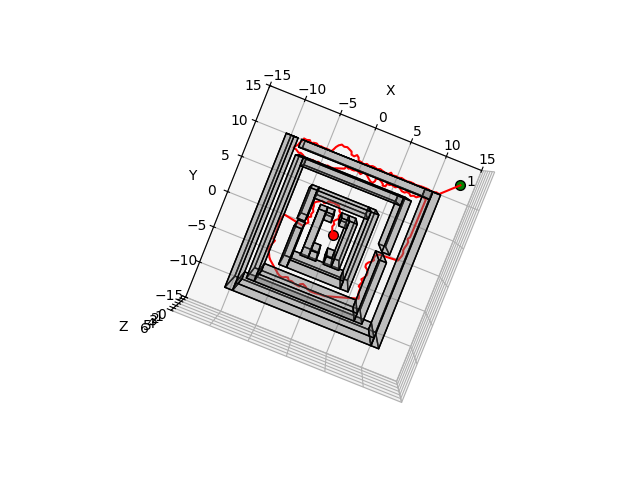
\includegraphics[width=0.7\columnwidth]{test_maze.png}}
    \caption{Trajectory overcoming bug traps in the Maze environment.}
    \label{fig:maze}
\end{figure}

\begin{figure}[htbp]
    \centerline{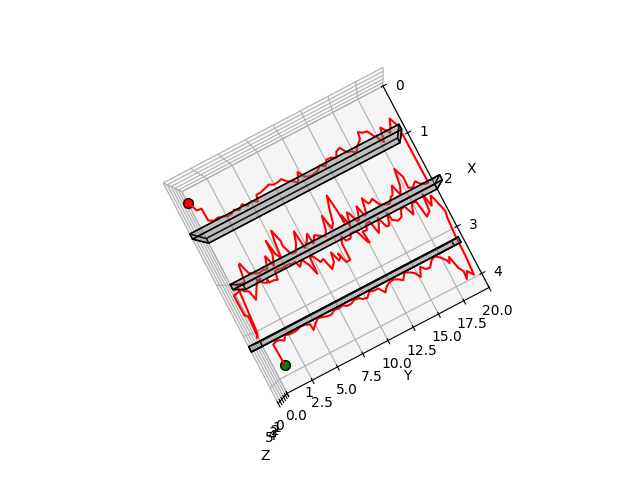
\includegraphics[width=0.7\columnwidth]{test_monza.png}}
    \caption{Trajectory through the highly constrained Monza environment.}
    \label{fig:monza}
\end{figure}

\subsection{Dynamic Goal Environments}
For the dynamic environments (Window and Room), the target moves through eight sequential positions. The planner computed paths from scratch for each transition. Table \ref{tab:dynamic_results} details the execution time and path length for each of the eight sequential goals.

\begin{table}[htbp]
    \caption{Performance in Dynamic Environments (Sequential Goals 1 to 8)}
    \begin{center}
        \begin{tabular}{|c|c|c|c|c|}
            \hline
                          & \multicolumn{2}{c|}{\textbf{Window}} & \multicolumn{2}{c|}{\textbf{Room}}                                     \\
            \hline
            \textbf{Goal} & \textbf{Time (s)}                    & \textbf{Path}                      & \textbf{Time (s)} & \textbf{Path} \\
            \hline
            1             & 0.016                                & 22.94                              & 0.009             & 4.84          \\
            \hline
            2             & 0.008                                & 22.71                              & 0.006             & 10.01         \\
            \hline
            3             & 0.005                                & 22.95                              & 0.006             & 9.97          \\
            \hline
            4             & 0.009                                & 25.34                              & 0.004             & 5.83          \\
            \hline
            5             & 0.008                                & 26.01                              & 0.008             & 11.55         \\
            \hline
            6             & 0.009                                & 23.62                              & 0.008             & 15.44         \\
            \hline
            7             & 0.008                                & 25.43                              & 0.011             & 13.57         \\
            \hline
            8             & 0.006                                & 20.23                              & 0.033             & 23.30         \\
            \hline
        \end{tabular}
        \label{tab:dynamic_results}
    \end{center}
\end{table}

Because the maximum computation time observed across all dynamic queries is only 0.033 seconds, the planner satisfies the dynamic replanning constraints with a massive margin. Based on these empirical results, the minimum achievable total time period (calculated as $t_1 + 7t_2$) is $0.32$ seconds, assuming optimal bounding limits of $t_1 = 0.04$ and $t_2 = 0.04$ seconds.

Figures \ref{fig:window} and \ref{fig:room} visualize the sequential paths capturing the moving targets.

\begin{figure}[htbp]
    \centerline{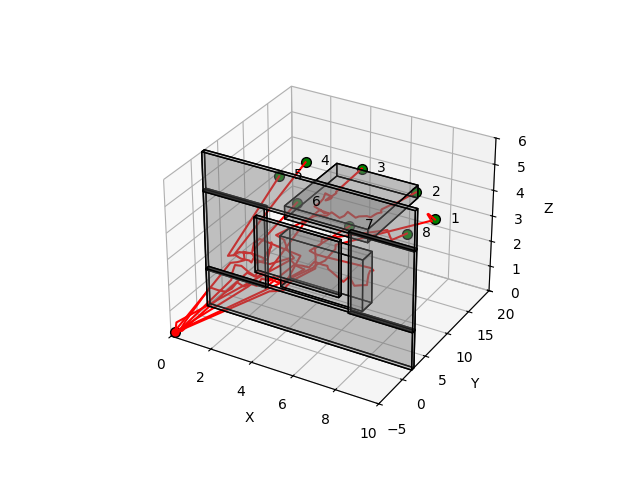
\includegraphics[width=0.7\columnwidth]{test_window.png}}
    \caption{Sequential interception paths in the Window environment.}
    \label{fig:window}
\end{figure}

\begin{figure}[htbp]
    \centerline{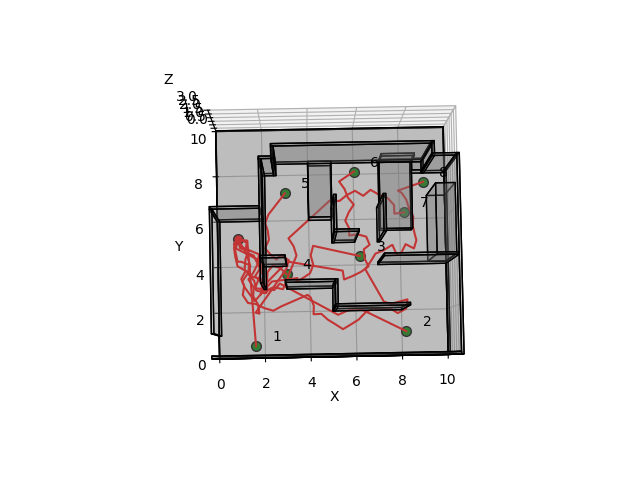
\includegraphics[width=0.7\columnwidth]{test_room.png}}
    \caption{Sequential interception paths in the Room environment.}
    \label{fig:room}
\end{figure}

\subsection{Discussion of Algorithmic Performance and Challenges}
During the development and testing phases, several engineering challenges and algorithmic trade offs were encountered and successfully resolved. We outline the key findings below:

\textbf{1. Dynamic Constraints and Goal-Biased Sampling:}
To satisfy the extreme dynamic replanning limits, we initially implemented a unidirectional RRT with a goal-biased sampling strategy paired with a fully vectorized Slab Method. Implementing this required careful tuning of the bias probability parameter. If the bias was set too high (e.g., above 10 percent), the algorithm acted as a greedy local planner and lost its space exploring capabilities, getting stuck on trivial obstacles. If set too low, it degraded into vanilla RRT and failed the 0.1 second replanning limit. We empirically found that a 2 percent goal bias offered the optimal trade off. Furthermore, strict step size constraints had to be enforced when the goal was sampled, ensuring the tree only extended by a single step toward the goal rather than attempting a direct, collision prone connection across the map.

\textbf{2. Overcoming Bug Traps in the Maze:}
When tested in the highly constrained Maze environment, the initial goal-biased planner repeatedly fell into bug traps, exhausting its iteration limits by attempting to penetrate solid walls toward the goal. Transitioning to the Bi-Directional RRT-Connect architecture completely resolved this vulnerability. The dual tree structure and greedy bidirectional connection heuristic naturally guided the search out of dead ends.

\textbf{3. Node Exhaustion and Step Size Tuning:}
Early tests with the bidirectional planner in the Maze revealed that a limit of 20000 nodes was exhausted in merely 1.2 seconds, indicating insufficient node density. Leveraging the extreme efficiency of our vectorized collision checking, we expanded the maximum iteration limit to 100000 and subtly reduced the step size from 0.5 to 0.4. This fine tuning allowed the tree to densely explore and successfully navigate narrow corridors.

\textbf{4. Path Reconstruction Artifacts:}
During development, we observed an anomaly where the final visualized path would occasionally contain a massive segment penetrating through obstacles. This was identified as a topological logic error during array splicing when the two trees swapped and connected. Implementing a strict array reversal operation prior to concatenation seamlessly eliminated these phantom collisions.

\textbf{5. Trajectory Suboptimality and Path Smoothing:}
In open environments, the generated trajectories occasionally exhibited jagged, knot like patterns. This visual artifact is a fundamental characteristic of uniform random sampling. While the RRT algorithm guarantees probabilistic completeness, it does not guarantee optimality. For real world physical robotic deployments, introducing a post processing path smoothing step would be necessary to straighten and optimize these suboptimal trajectory segments.

\end{document}